\documentclass[tikz]{standalone}
\begin{document}
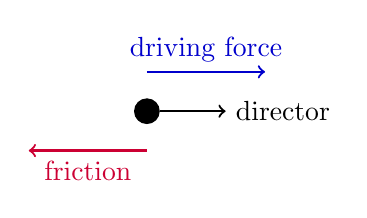
\begin{tikzpicture}[thick]
  \node[draw,fill,circle,inner sep=3pt] (A) {};
  \draw[->] (A) -- ++(1,0) node[right] {director};
  \draw[blue!80!black,->] (A) ++(0, .5) -- node[above] {driving force} ++(1.5,0);
  \draw[red!80!blue,->] (A) ++(0,-.5) -- node[below] {friction} ++(-1.5,0);
\end{tikzpicture}
\end{document}
